
As Figuras \ref{fig:TT170TP375micros} a \ref{fig:TT170TP450micros} mostram micrografias das microestruturas das amostras temperadas a \SI{170}{\degreeCelsius} e particionadas a 200, 250, 300, 375 e \SI{450}{\degreeCelsius} por 15 minutos. Nesta análise a temperatura de têmpera foi mantida fixa para que apenas o efeito da temperatura de partição fosse levado em conta. Dessa forma, as quantidades de martensita são as mesmas na análise destas amostras. Como apresentado na metodologia do trabalho, o ataque seletivo empregado na avaliação por microscopia óptica tinge tanto a ferrita quanto a martensita, enquanto as áreas em branco --- em que não há deposição do reagente --- são atribuídas à austenita retida e carbonetos. Quanto à análise por microscopia eletrônica, o ataque por Nital também consume preferencialmente ferrita e austenita, enquanto regiões de austenita aparecem em alto relevo. 

As imagens obtidas por MO das amostras particionadas a 300 e \SI{375}{\degreeCelsius} (Figuras \ref{fig:TT170TP300micros}a e \ref{fig:170TP375micros}a) revela produtos alongados tingidos, ora na forma de placas grossas, ora na forma de um produto mais fino, intercalados por blocos poligonais brancos; alguns nódulos de grafita também podem ser vistos na magnificação empregada. As regiões brancas são correspondentes à austenita retida enriquecida em carbono pelo processo T\&P. Por sua vez, a morfologia de placas é natural de martensita formada em ligas de alto carbono (em oposição à morfologia em ripas da martensita em baixo carbono), enquanto as finas agulhas são relacionadas ao produto ferrítico da reação bainítica.

\begin{figure}
  \centering
  \subfloat[]{%
    \begin{minipage}[c][.4\textwidth]{.50\textwidth}
      \centering%
      \includegraphics[width=\textwidth]{img/micrografias/MO/TT170TP375/1000x-1.pdf}
    \end{minipage}}
  \quad
  \subfloat[]{%
    \begin{minipage}[c][.4\textwidth]{.47\textwidth}
      \centering%
      %\includegraphics[width=\textwidth]{img/micrografias/MEV/TT170TP375/10k-2}
      \includegraphics[width=\textwidth]{img/micrografias/MEV/TT170TP375/25k-4}
    \end{minipage}}
  \caption{Amostra T\&P, $T_T$ = \SI{170}{\degreeCelsius}, $T_P$ = \SI{375}{\degreeCelsius} / 15 minutos. (a) MO, aumento de 1000x. Áreas brancas são correspondentes a regiões de $\gamma$, enquanto regiões tingidas correspondem a $\alpha$ (b) MEV, aumento de 25kx. É possível observar detalhe da martensita em morfologia de placas (alto carbono) e do produto isotérmico, indicados, respectivamente, pelas setas azul e vermelha. Rugosidade observada na martensita parece ser um artefato de ataque.}
  \label{fig:TT170TP375micros}
\end{figure}

\begin{figure}
  \centering
  \subfloat[]{%
    \begin{minipage}[c][.4\textwidth]{.50\textwidth}
      \centering%
      \includegraphics[width=\textwidth]{img/micrografias/MO/TT170TP300/1000x-2.pdf}
    \end{minipage}}
  \quad
  \subfloat[]{%
    \begin{minipage}[c][.4\textwidth]{.47\textwidth}
      \centering%
      \includegraphics[width=\textwidth]{img/micrografias/MEV/TT170TP300/25k-2.pdf}
    \end{minipage}}
  \caption{Amostra T\&P, $T_T$ = \SI{170}{\degreeCelsius}, $T_P$ = \SI{300}{\degreeCelsius} / 15 minutos. (a) MO, aumento de 1000x. Áreas brancas são correspondentes a regiões de $\gamma$, enquanto regiões tingidas correspondem a $\alpha$ (b) MEV, aumento de 25kx. Produto isotérmico, indicado pelas setas vermelhas, é mais refinado do que o formado a \SI{375}{\degreeCelsius}.}
  \label{fig:TT170TP300micros}
\end{figure}

A caracterização dos aspectos microestruturais fica no limite de resolução do microscópio óptico. As imagens obtidas por MEV mostradas nas Figuras \ref{fig:TT170TP300micros}b e \ref{fig:TT170TP375micros}b apresentam grande maior de detalhes. A partir delas pode-se distinguir com clareza a martensita do produto bainítico, indicados, respectivamente, por setas azuis e vermelhas. Além disso, apesar de à luz do microscópio óptico as duas microestruturas sejam bastante semelhantes, a partir da análise por MEV verifica-se nitidamente que o produto pró-bainítico formado a \SI{300}{\degreeCelsius} é mais refinado do que aquele formado a \SI{375}{\degreeCelsius}.

A amostra particionada a \SI{300}{\degreeCelsius} observada no microscópio sob baixa magnificação (Figura \ref{fig:TT170TP300-100x}) mostra que as áreas brancas de austenita retida não são distribuídas homogeneamente ao longo do material. Na verdade, observam-se porções em que há predominância de austenita retida, como indicam os retângulos vermelhos na figura. Isso é provavelmente devido à segregação de elementos de liga remanescente da solidificação e, portanto, essas áreas são associadas aos antigos contornos de célula eutética. Esse mesmo comportamento foi observado nas demais amostras tratadas termicamente.

\begin{figure}
  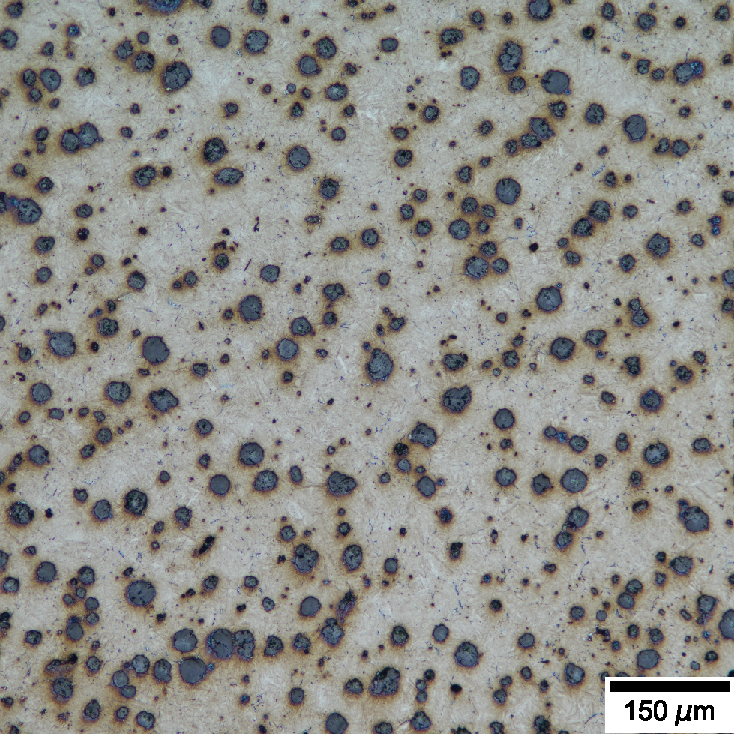
\includegraphics[width=.7\textwidth]{img/micrografias/MO/TT170TP300/100x-1.pdf}
  \caption{Amostra T\&P, $T_T$ = \SI{170}{\degreeCelsius}, $T_P$ = \SI{300}{\degreeCelsius} / 15 minutos, aumento de 100x. Os retângulos vermelhos destacam algumas áreas brancas com maior predominância de austenita retida, correspondentes aos antigos contornos de célula eutética.}
  \label{fig:TT170TP300-100x}
\end{figure}

A descrição da microestrutura da amostra particionada a \SI{250}{\degreeCelsius} (Figura \ref{fig:TT170TP250micros}) é semelhante a das amostras particionadas a 300 e \SI{375}{\degreeCelsius}. Na imagem de MO (Figura \ref{fig:TT170TP250micros}a) também são observadas placas de martensita, produtos aciculares --- novamente associados ao produto bainítico --- e regiões brancas, que a princípio poderiam ser interpretadas novamente como austenita. Todavia, tendo em vista a estabilidade da austenita produzida nesta condição, é provável que estas regiões na verdade correspondam a uma mistura de austenita e martensita fresca produzida durante o resfriamento final (indicado pela inflexão a \SI{77}{\degreeCelsius} nos ensaios de dilatometria). Este tipo de microestrutura é, principalmente na literatura de aços Alta Resistência e Baixa Liga (ARBL), denominado microconstituinte MA (martensita + austenita). Embora, regiões de MA contenham martensita, que em tese deveria ser tingida pelo reagente metalográfico, este microconstituinte é inerte ao reagente seletivo. %REFERÊNCIAS!

\begin{figure}
  \centering
  \subfloat[]{%
    \begin{minipage}[c][.4\textwidth]{.50\textwidth}
      \centering%
      \includegraphics[width=\textwidth]{img/micrografias/MO/TT170TP250/1000x-2.pdf}
    \end{minipage}}
  \quad
  \subfloat[]{%
    \begin{minipage}[c][.4\textwidth]{.47\textwidth}
      \centering%
      \includegraphics[width=\textwidth]{img/micrografias/MEV/TT170TP250/25k-1.pdf}
    \end{minipage}}
  \vspace{0pt}
  \subfloat[]{%
    \begin{minipage}[c][.48\textwidth]{.57\textwidth}
      \centering%
      \includegraphics[width=\textwidth]{img/micrografias/MEV/TT170TP250/50k-4.pdf}
    \end{minipage}}
  \caption{Amostra T\&P, $T_T$ = \SI{170}{\degreeCelsius}, $T_P$ = \SI{250}{\degreeCelsius} / 15 minutos. (a) MO, aumento de 1000x. (b) MEV, aumento de 25kx. (c) MEV, aumento 50kx. A fração volumétrica do produto isotérmico (setas vermelhas) é menor do que nas condições anteriores. O produto também parecer ser ainda mais refinado.}
  \label{fig:TT170TP250micros}
\end{figure}

Sobre do produto bainítico formado a \SI{250}{\degreeCelsius}, novamente apenas observação por MEV permitiu uma caracterização adequada (Figuras \ref{fig:TT170TP250micros}b e \ref{fig:TT170TP250micros}c). Nota-se que sua fração volumétrica é significativamente menor, como previsto pelos resultados de dilatometria, e que é mais refinado que aquele formado em temperaturas mais elevadas.
%Em comparação às imagens das amostras particionadas a \SI{300}{\degreeCelsius}, nota-se que o produto produzido a \SI{250}{\degreeCelsius} é mais refinado e é de difícil interpretação apenas por microscopia óptica.

A Figura \ref{fig:TT170TP200micros} mostra as micrografias da amostra temperada particionada a \SI{200}{\degreeCelsius} por 15 min, após têmpera a \SI{170}{\degreeCelsius}. Ao contrário das condições anteriores, nas magnificações permitidas pelo MO e pelo MEV não são observados produtos aciculares que possam ser associados à reação bainítica. De fato, após apenas 15 minutos de partição, os resultados de DRX e dilatometria mostram que a fração transformada é muito pequena. Além disso, a austenita obtida não é estável, o que é refletido na formação de martensita durante o resfriamento final. 

\begin{figure}
  \centering
  \subfloat[]{%
    \begin{minipage}[c][.4\textwidth]{.50\textwidth}
      \centering%
      \includegraphics[width=\textwidth]{img/micrografias/MO/TT170TP200/1000x-1.pdf}
    \end{minipage}}
  \quad
  \subfloat[]{%
    \begin{minipage}[c][.4\textwidth]{.47\textwidth}
      \centering%
      \includegraphics[width=\textwidth]{img/micrografias/MEV/TT170TP200/25k-2.pdf}
    \end{minipage}}
  \caption{Amostra T\&P, $T_T$ = \SI{170}{\degreeCelsius}, $T_P$ = \SI{200}{\degreeCelsius} / 15 minutos. (a) MO, aumento de 1000x. (b) MEV, aumento de 25kx. Não é possível identificar os produtos aciculares observados para temperaturas mais elevadas de partição, apenas placas de martensita.}
  \label{fig:TT170TP200micros}
\end{figure}

No entanto, para duas horas de partição a \SI{200}{\degreeCelsius}, as microestruturas se parecem mais com as das demais condições (Figura \ref{fig:TT170TP2002hmicros}). Fica evidenciada a coexistência de placas de martensita e um produto acicular mais fino do que o primeiro --- que parece ser tão refinado quanto aquele formado a \SI{250}{\degreeCelsius} ---, além de áreas em alto relevo correspondentes à austenita. A presença do microconstituinte acicular é novamente justificada por uma reação de decomposição da austenita durante a partição. Contudo, concluir que esse produto se trata de um constituinte pró-bainítico seria controverso, haja vista que a temperatura de \SI{200}{\degreeCelsius} é abaixo da temperatura Ms da liga (\SI{230}{\degreeCelsius}). De fato, na imagem obtida sob aumento de 25 mil vezes (Figura \ref{fig:TT170TP2002hmicros}c) observa-se que o crescimento dos produtos aciculares segue um padrão em ``zigue-zague'', tal qual é observado em algumas martensitas de alto carbono. Nestas martensitas, isto é justificado pela auto-catálise no crescimento das placas. Quando uma placa atinge um contorno de grão, imediatamente nucleia outra placa, que cresce para dentro do grão respeitando as relações de orientação cristalográfica.

\begin{figure}
  \centering
  \subfloat[]{\includegraphics[width=.48\textwidth]{img/micrografias/MEV/TT170TP200-2h/10k-1.pdf}}
  \quad
  \subfloat[]{\includegraphics[width=.48\textwidth]{img/micrografias/MEV/TT170TP200-2h/25k-1.pdf}}
  \caption{Amostra T\&P, $T_T$ = \SI{170}{\degreeCelsius}, $T_P$ = \SI{200}{\degreeCelsius} / 2h. (a) MEV, aumento de 10kx. (b) MEV, aumento de 25kx. As setas azuis indicam as placas de martensita e as setas vermelhas o produto isotérmico. O retângulo vermelho destaca uma região em que o produto isotérmico cresceu em ``zigue-zague''}
  \label{fig:TT170TP2002hmicros}
\end{figure}

%Na amostra particionada a \SI{450}{\degreeCelsius} (Figura \ref{fig:TT170TP450micros}), embora os resultados de dilatometria e difração de raios X mostrem que houve uma 
%não tenham sido quantificados frações volumétricas de austenita pela difração de raios X, observam-se regiões brancas nas regiões de contornos de célula eutética (setas vermelhas). A natureza desse produto, no entanto, não pode ser determinada nas magnificações permitidas pelo microscópio óptico.

Finalmente, as micrografias relativas à amostra particionada a \SI{450}{\degreeCelsius} são mostradas na Figura \ref{fig:TT170TP450micros}. Na imagem de MO (Figura \ref{fig:TT170TP450micros}a) a microestrutura é predominantemente tingida de azul pelo reagente metalográfico, indicando grande quantidade de martensita e ferrita. No entanto, embora os resultados de DRX mostrarem que após 15 minutos de partição a austenita foi consumida praticamente em sua totalidade, a imagem também revela algumas regiões brancas que poderiam ser associadas a essa fase, aparentemente concentradas nas regiões segregadas de contorno de célula. As imagens de microscopia eletrônica, mostradas nas Figuras \ref{fig:TT170TP450micros}b e \ref{fig:TT170TP450micros}c, parecem confirmar esta hipótese, ao mostrar áreas poligonais em alto relevo, compatíveis com a descrição morfológica da austenita.

\begin{figure}
  \centering
  \subfloat[]{%
    \begin{minipage}[c][.4\textwidth]{.50\textwidth}
      \centering%
      \includegraphics[width=\textwidth]{img/micrografias/MO/TT170TP450/1000x-1.pdf}
    \end{minipage}}
  \quad
  \subfloat[]{%
    \begin{minipage}[c][.4\textwidth]{.47\textwidth}
      \centering%
      \includegraphics[width=\textwidth]{img/micrografias/MEV/TT170TP450/10k-8.pdf}
    \end{minipage}}
  \vspace{0pt}
  \subfloat[]{%
    \begin{minipage}[c][.48\textwidth]{.57\textwidth}
      \centering%
      \includegraphics[width=\textwidth]{img/micrografias/MEV/TT170TP450/25k-1.pdf}
    \end{minipage}}
  \caption{Amostra T\&P, $T_T$ = \SI{170}{\degreeCelsius}, $T_P$ = \SI{450}{\degreeCelsius} / 15 minutos. (a) MO, aumento de 1000x. (b) MEV, aumento de 10kx. (c) MEV, aumento de 25kx. As setas verdes indicam as regiões com maior quantidade de austenita retida, em contornos de célula eutética. As setas azuis indicam as placas de martensita.}
  \label{fig:TT170TP450micros}
\end{figure}

Diferentemente das demais condições de partição, as imagens de MEV revelam um fina dispersão de precipitados ao longo de todo o material particionado a \SI{450}{\degreeCelsius}. Pelo já discutido nos resultados de dilatometria, é possível concluir que se tratam de carbonetos provenientes do segundo estágio da reação bainítica e do revenimento da martensita. Para duas horas de partição, essa dispersão de precipitados fica ainda mais evidente, como mostra a Figura \ref{fig:TT170TP4502hmicros}. Na Figura \ref{fig:TT170TP4502hmicros}b, que mostra o detalhe de uma placa de martensita, se percebe uma distribuição muita fina de partículas em seu interior. 

\begin{figure}
  \subfloat[]{\includegraphics[width=.48\textwidth]{img/micrografias/MEV/TT170TP450-2h/10k-1.pdf}}
  \quad
  \subfloat[]{\includegraphics[width=.48\textwidth]{img/micrografias/MEV/TT170TP450-2h/50k-1.pdf}}
  \caption{Amostra T\&P, $T_T$ = \SI{170}{\degreeCelsius}, $T_P$ = \SI{450}{\degreeCelsius} / 2h. (a) MEV, aumento de 10kx. O retângulo azul indica a região em que foi obtido (b) MEV, aumento de 50kx. Observa dispersão muito fina de carbonetos no interior da placa de martensita.}
  \label{fig:TT170TP4502hmicros}
\end{figure}

Ou seja, pode-se dizer que nessa condição ocorre a decomposição eutetóide da austenita ($\gamma \rightarrow \alpha + \theta$) durante a partição, com a formação de bainita convencional.